%CHAPTER
\chapter{Implementace modulu}

\section{Generátor}
%SUBSECTION
\subsection{TCPDF x mPDF}
%vyhody nevyhody, výsledný názoromezení, chyby knihovny ((popis doimplementování našeho kódu)), 

\begin{figure}[h!]
\centering
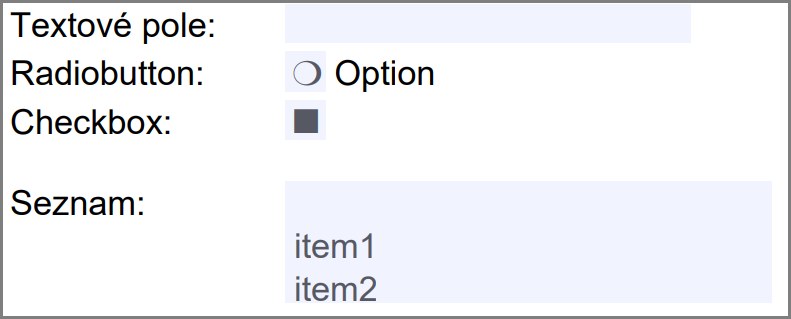
\includegraphics[width=8cm]{img/tcpdf_elements}
\caption{Formulářové prvky vytvořené pomocí TCPDF}
\label{fig:tcpdf_elements}
\end{figure}

\begin{lstlisting}[caption = {Zdrojový kód psaný v PHP využívající knihovnu TCPDF}, label = {lst:tcpdf_code}, captionpos=b]
    <?php
    require_once($_SERVER['DOCUMENT_ROOT'] . '/TSD/lib/tcpdf/tcpdf.php');
    $pdf = new TCPDF(PDF_PAGE_ORIENTATION, PDF_UNIT, PDF_PAGE_FORMAT, TRUE, 'UTF-8', FALSE);
    $pdf->SetAutoPageBreak(TRUE, PDF_MARGIN_BOTTOM);
    $pdf->AddPage();
    $pdf->Cell(35, 5, 'Textove pole:');
    $pdf->TextField('firstname', 50, 5);
    $pdf->Ln(6);
    $pdf->Cell(35, 5, 'Radiobutton:');
    $pdf->RadioButton('drink', 5, array(), array(), 'Water');
    $pdf->Cell(35, 5, 'Option');
    $pdf->Ln(6);
    $pdf->Cell(35, 5, 'Checkbox:');
    $pdf->CheckBox('newsletter', 5, true, array(), array(), 'OK');
    $pdf->Ln(10);
    $pdf->Cell(35, 5, 'Seznam:');
    $pdf->ListBox('listbox', 60, 15, array('', 'item1', 'item2', 'item3', 'item4'), array('multipleSelection'=>'true'));
    $pdf->Ln(20);            
    $pdf->Output();
    ?>
\end{lstlisting}

\begin{figure}[h!]
\centering
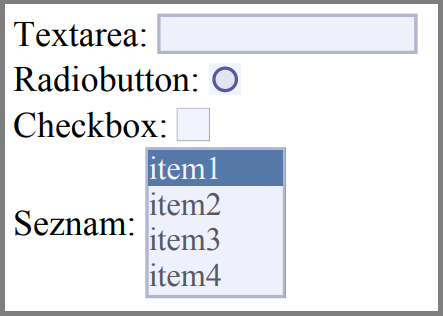
\includegraphics[width=5cm]{img/mpdf_elements}
\caption{Formulářové prvky vytvořené pomocí mPDF}
\label{fig:mpdf_elements}
\end{figure}

\begin{lstlisting}[caption = {Zdrojový kód psaný v PHP využívající knihovnu mPDF}, label = {lst:mpdf_code}, captionpos=b]
    <?php
    require_once($_SERVER['DOCUMENT_ROOT'] . '/TSD/lib/mpdf/vendor/autoload.php');
    $pdf = new \Mpdf\Mpdf(); 
    $pdf->useActiveForms = true;        
    $html = 'Textarea:    <textarea name="message" rows="1" cols="10">a</textarea>
            <br>
            Radiobutton: <input type="radio" name="radio" value="radio">
            <br>
            Checkbox:    <input type="checkbox" name="checkbox" value="checkbox">
            <br>
            Seznam:
            <select name="select" size="4">
                <option value="option1">item1</option>
                <option value="option2">item2</option>
                <option value="option3">item3</option>
                <option value="option4">item4</option>
            </select>
            ';

    $pdf->WriteHTML($html, 2);
    $pdf->Output();
    ?>
\end{lstlisting}

\section{Parser}
%omezení, chyby knihovny, dosáhnutí výsledků (popis doimplementování našeho kódu)

\section{Implementované třídy}
%popis důležitých funkcí

\section{Výsledný vzhled PDF formuláře}
 %

